\documentclass[paper=a4, fontsize=11pt]{scrartcl} % A4 paper and 11pt font size

\usepackage[T1]{fontenc} % Use 8-bit encoding that has 256 glyphs
\usepackage{fourier} % Use the Adobe Utopia font for the document - comment this line to return to the LaTeX default
\usepackage[english]{babel} % English language/hyphenation
\usepackage{amsmath,amsfonts,amsthm} % Math packages
\usepackage{graphicx}
\usepackage{lipsum} % Used for inserting dummy 'Lorem ipsum' text into the template

\usepackage{sectsty} % Allows customizing section commands
\allsectionsfont{\centering \normalfont\scshape} % Make all sections centered, the default font and small caps

\usepackage{fancyhdr} % Custom headers and footers
\pagestyle{fancyplain} % Makes all pages in the document conform to the custom headers and footers
\fancyhead{} % No page header - if you want one, create it in the same way as the footers below
\fancyfoot[L]{} % Empty left footer
\fancyfoot[C]{} % Empty center footer
\fancyfoot[R]{\thepage} % Page numbering for right footer
\renewcommand{\headrulewidth}{0pt} % Remove header underlines
\renewcommand{\footrulewidth}{0pt} % Remove footer underlines
\setlength{\headheight}{13.6pt} % Customize the height of the header

\numberwithin{equation}{section} % Number equations within sections (i.e. 1.1, 1.2, 2.1, 2.2 instead of 1, 2, 3, 4)
\numberwithin{figure}{section} % Number figures within sections (i.e. 1.1, 1.2, 2.1, 2.2 instead of 1, 2, 3, 4)
\numberwithin{table}{section} % Number tables within sections (i.e. 1.1, 1.2, 2.1, 2.2 instead of 1, 2, 3, 4)

\setlength\parindent{0pt} % Removes all indentation from paragraphs - comment this line for an assignment with lots of text

%----------------------------------------------------------------------------------------
%       TITLE SECTION
%----------------------------------------------------------------------------------------

\newcommand{\horrule}[1]{\rule{\linewidth}{#1}} % Create horizontal rule command with 1 argument of height

\title{
\normalfont \normalsize
\textsc{Jiangsu University, school of Computer Science and Communication Engineering} \\ [25pt] % Your university, school and/or department name(s)
\horrule{0.5pt} \\[0.4cm] % Thin top horizontal rule
\huge Cryptography\_exercises \\ % The assignment title
\horrule{2pt} \\[0.5cm] % Thick bottom horizontal rule
}

\author{Zhendong Yang} % Your name

\date{\normalsize\today} % Today's date or a custom date

\begin{document}

\maketitle % Print the title

\section{Key Management}
\label{sec:km}


\textbf{1.} One local area network vendor provides a key distribution facility, as illustrated in Figure \ref{7-3}.

\begin{enumerate}
\item Describe the scheme.
\item Compare this scheme to that of Figure \ref{7-4}. What are the pros and cons?
\end{enumerate}

\begin{figure}[htbp]
  \centering
  \includegraphics[width=7cm]{7-3.eps}
  \caption{Figure for problem 7.1}
  \label{7-3}
\end{figure}

\begin{figure}[htbp]
  \centering
  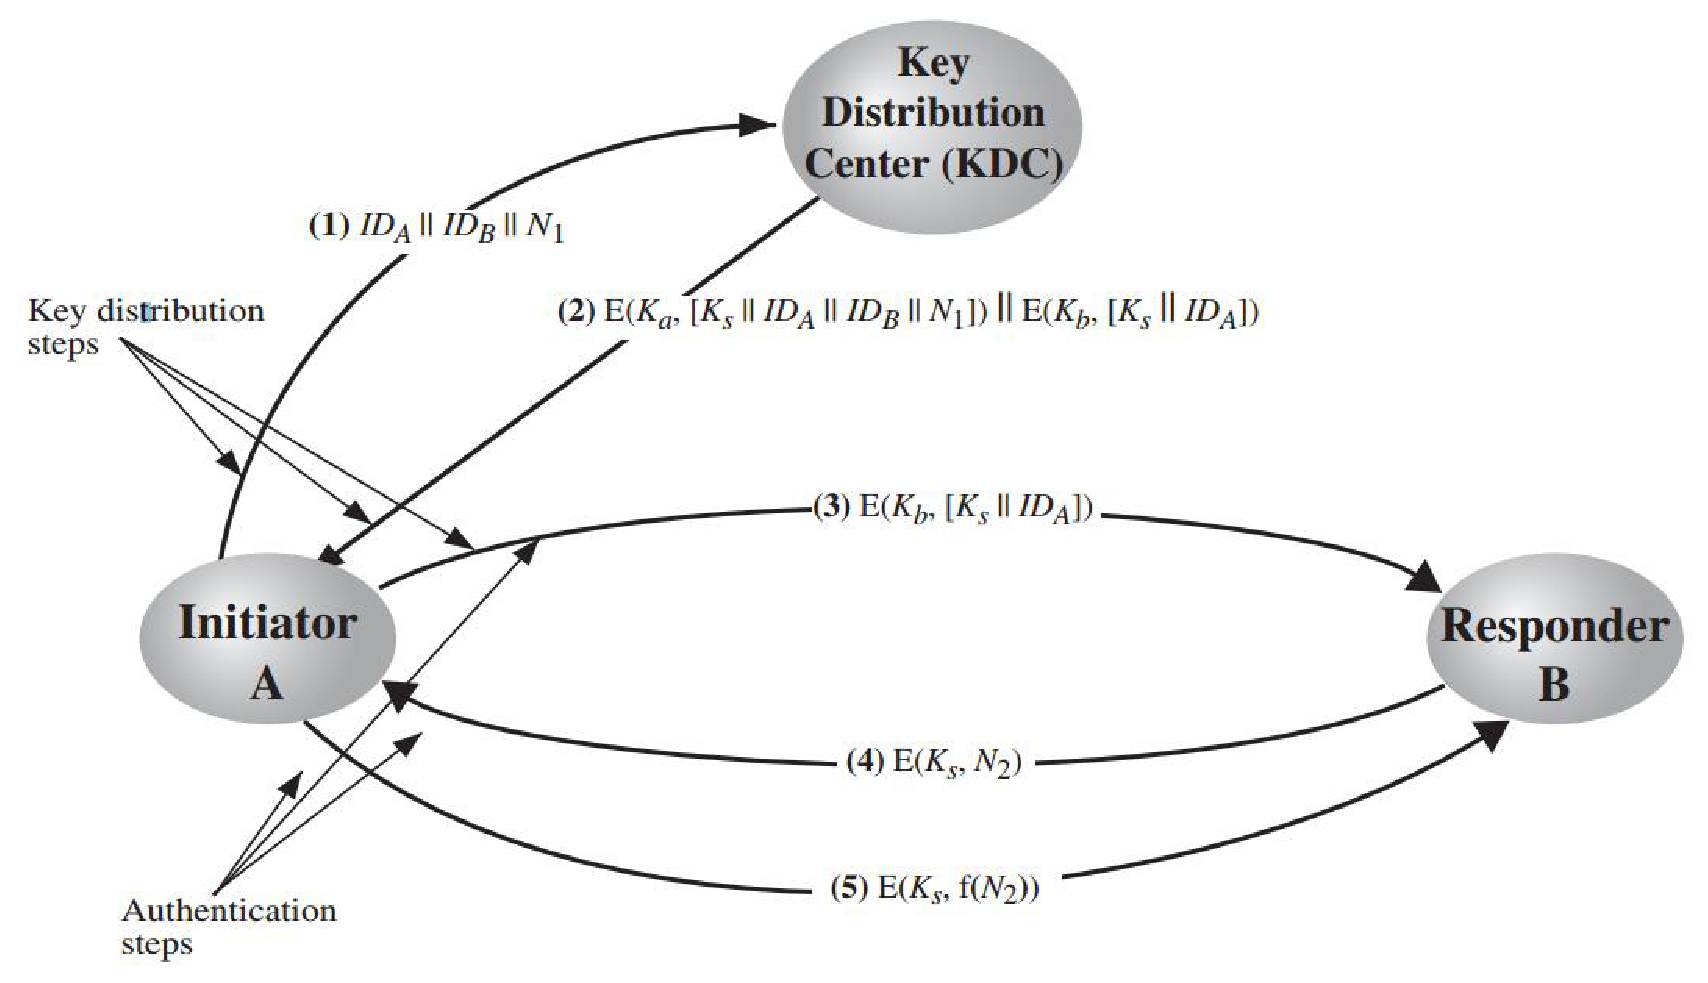
\includegraphics[width=7cm]{7-4.eps}
  \caption{Key distribution scenario}
  \label{7-4}
\end{figure}

\textbf{Answer:}

\begin{enumerate}
\item A sends a connection request to B, with an event marker or nonce (Na) encrypted with the key that A shares with the KDC. If B is prepared to accept the connection, it sends a request to the KDC for a session key, including A's encrypted nonce plus a nonce generated by B (Nb) and encrypted with the key that B shares with the KDC. The KDC returns two encrypted blocks to B. One block is intended for B and includes the session key, A's identifier, and B's nonce. A similar block is prepared for A and passed from the KDC to B and then to A. A and B have now securely obtained the session key and, because of the nonces, are assured that the other is authentic.
\item The proposed scheme appears to provide the same degree of security as that of Figure \ref{7-4}. One advantage of the proposed scheme is that the, in the event that B rejects a connection, the overhead of an interaction with the KDC is avoided.
\end{enumerate}

\textbf{2.} What is the purpose of the X.509 standard?\\

\textbf{Answer:}

X.509 defines a framework for the provision of authentication services by the X.500 directory to its users. The directory may serve as a repository of public-key
certificates. Each certificate contains the public key of a user and is signed with the private key of a trusted certification authority.\\

\textbf{3.} The 1988 version of X.509 lists properties that RSA keys must satisfy to be secure given current knowledge about the difficulty of factoring large numbers. The discussion concludes with a constraint on the public exponent and the modulus $n$:

\begin{enumerate}
\item[-] It must be ensured that $e > \log_{2}(n) $ to prevent attack by taking the $e$th root mod $n$ to disclose the plaintext.
\end{enumerate}

Although the constraint is correct, the reason given for requiring it is incorrect. What is wrong with the reason given and what is the correct reason?\\

\textbf{Answer:}

Taking the $e$th root mod $n$ of a ciphertext block will always reveal the plaintext, no matter what the values of $e$ and $n$ are. In general this is a very difficult problem, and indeed is the reason why RSA is secure. The point is that, if $e$ is too small, then taking the normal integer eth root will be the same as taking the $e$th root mod $n$, and taking integer $e$th roots is relatively easy.


\textbf{4.} List ways in which secret keys can be distributed to two communicating parties.\\

\textbf{Answer:}

For two parties A and B, key distribution can be achieved in a number of ways, as
follows:

\begin{enumerate}
\item A can select a key and physically deliver it to B.
\item A third party can select the key and physically deliver it to A and B.
\item If A and B have previously and recently used a key, one party can transmit the new key to the other, encrypted using the old key.
\item If A and B each has an encrypted connection to a third party C, C can deliver a key on the encrypted links to A and B.
\end{enumerate}


\textbf{5.} NIST defines the term cryptoperiod as the time span during which a specific key is authorized for use or in which the keys for a given system or application may remain in effect. One document on key management uses the following time diagram for a shared secret key.

\begin{figure}[htbp]
  \centering
  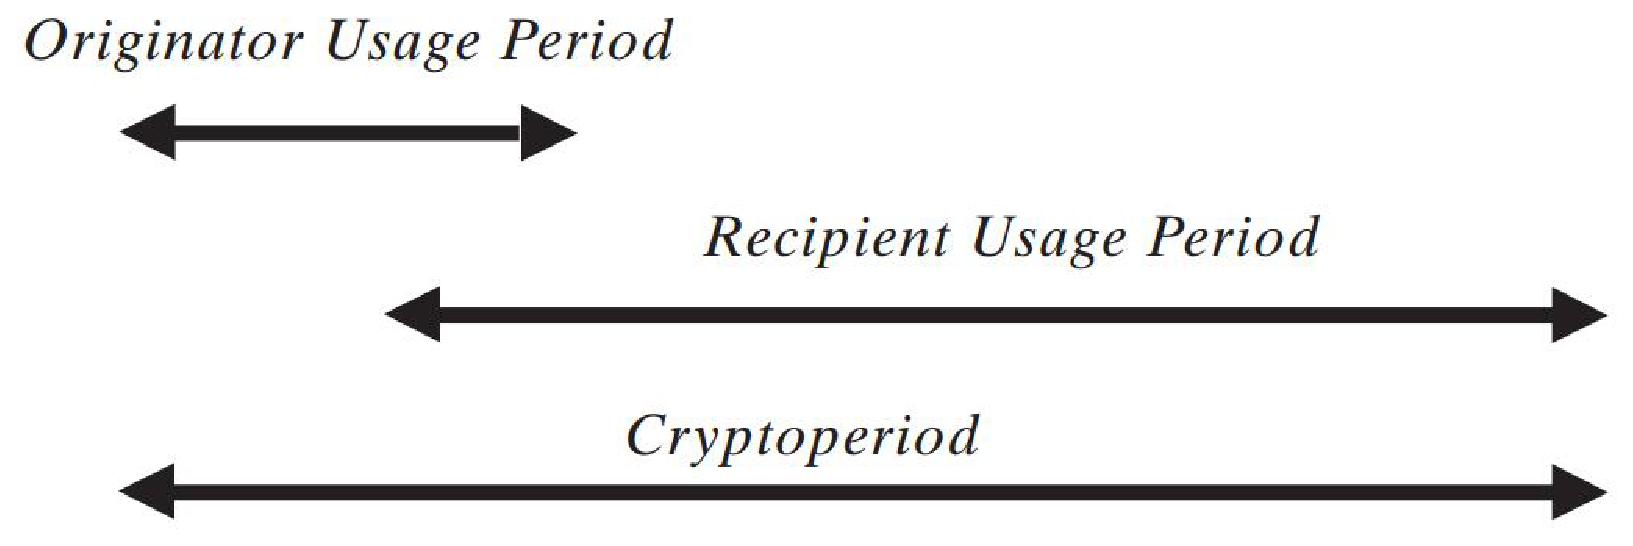
\includegraphics[width=7cm]{7-5.eps}
  \caption{Time diagram for a shared secret key}
  \label{7-5}
\end{figure}

Explain the overlap by giving an example application in which the originator��s usage period for the shared secret key begins before the recipient��s usage period and also ends before the recipients usage period.\\

\textbf{Answer:}

When a symmetric key is used to protect stored information, the recipient usage period may start after the beginning of the originator usage period as shown in the figure. For example, information may be encrypted before being stored on a compact disk. At some later time, the key may be distributed in order to decrypt and recover the information.\\


\textbf{6.} What are the core components of a PKI? Briefly describe each component.\\

\textbf{Answer:}

A typical PKI consists of seven core components. These are briefly described below:

\begin{enumerate}
\item Digital certificates (public-key certificates, X.509 certificates): A digital certificate is a signed data structure that binds one or more attributes of an entity with its corresponding public key. By being signed by a recognized and trusted authority (i.e. the Certification Authority) a digital certificate provides assurances that a particular public key belongs to a specific entity (and that the entity possesses the corresponding private key).
\item Certification Authority (CA): Certification Authorities are the people, processes and tools that are responsible for the creation, issue and management of public-key certificates that are used within a PKI.
\item Registration Authority (RA): Registration Authorities are the people, processes and tools that are responsible for authenticating the identity of new entities (users or computing devices) that require certificates from CAs. RAs additionally maintain local registration data and initiate renewal or revocation processes for old or redundant certificates. They act as agents of CAs (and in that regard can carry out some of the functions of a CA if required).
\item Certificate repository: A database, or other store, which is accessible to all users of a PKI, within which public-key certificates, certificate revocation information and policy information can be held.
\item PKI client software: Client-side software is required to ensure PKI-entities are able to make use of the key and digital certificate management services of a PKI (e.g. key creation, automatic key update and refreshment).
\item PKI-enabled applications: Software applications must be PKI-enabled before they can be used within a PKI. Typically this involves modifying an application so that it can understand and make use of digital certificates (e.g. to authenticate a remote user and authenticate itself to a remote user).
\item Policy (Certificate Policy and Certification Practice Statement): Certificate Policies and Certification Practice Statements are policy documents that define the procedures and practices to be employed in the use, administration and management of certificates within a PKI.
\end{enumerate}


\textbf{7.} Explain the problems with key management and how it affects symmetric cryptography.

\textbf{Note}: The remaining problems deal with the a cryptographic product developed by IBM, which is briefly described in a document at this book��s Web site (IBMCrypto.pdf). Try these problems after reviewing the document.\\

\textbf{Answer:}

The primary weakness of symmetric encryption algorithms is keeping the single key secure. Known as key management, it poses a number of significant challenges. If a user wants to send an encrypted message to another using symmetric encryption, he must be sure that she has the key to decrypt the message. How should the first user get the key to the second user? He would not want to send it electronically through the Internet, because that would make it vulnerable to eavesdroppers. Nor can he encrypt the key and send it, because the
recipient would need some way to decrypt the key. And if he can even get the get securely to the user, how can be he certain that an attacker has not seen the key on that person��s computer? Key management is a significant impediment to using symmetric encryption.\\


\textbf{8.} What is the effect of adding the instruction $EMK_i$

\centerline{$EMK_i: X \rightarrow E(KMH^i, X) i = 0, 1$}

\textbf{Answer:}

Adding $EMK_0$ would allow users to generate personal session keys, which could be exchanged, avoiding the necessity of storing a key variable in a user-to-user session.\\


\textbf{9.} The principal objective of the IBM Cryptographic Subsystem is to protect transmissions between a terminal and the processing system. Devise a procedure, perhaps adding instructions, which will allow the processor to generate a session key $KS$ and distribute it to Terminal $i$ and Terminal $j$ without having to store a key-equivalent variable in the host.\\

\textbf{Answer:}

One solution is to add an instruction similar to $RFMK$ of the form:

\centerline{$KEYGEN[RN, KMT_i, KMT_j]$}

which will interpret $RN$ as $E(KMH0, KS)$ and return both $E(KMHi, KS)$ and $E(KMHj, KS)$, which are sent to the terminals $i$ and $j$, respectively. $RN$ need not be maintained at the host.\\


\textbf{10.} Suppose $N$ different systems use the IBM Cryptographic Subsystem with host master keys $KMH[i](i=1,2,...N)$. Devise a method for communicating between systems without requiring the system to either share a common host master key or to divulge their individual host master keys.

\textbf{Hint}: each system needs three variants of its host master key.\\

\textbf{Answer:}

Host $i$ has master key $KMH_i$, with variants $KMH_i,j, j = 0, 1, 2$.

\begin{enumerate}
\item $KMH_{i,0}$: used to encrypt session key $KS$
\item $KMH_{i,1}$: used to encrypt user master keys (at Host $i$)
\item $KMH_{i,2}$:  used to encrypt cross domain key $KMH(i, j) = KMH(j, i)$ (Host $i$ to Host $j$)
\end{enumerate}

Host $i$ stores $E[KMH_{i,2}, KMH(i, j)]$ and uses a translation instruction $RFMK'$:

\begin{enumerate}
\item[-] $RFMK'[E[KMH_{i,2}, KMH(i, j)], E(KMH_{i,0}, KS)] �� E(KMH_{i,j}, K)]$
\end{enumerate}

A second translation function $RTMK$ (at Host $j$)

\begin{enumerate}
\item[-] $RTMK[E[KMH_{j,2}, KMH(j, i)], E(KMH(i, j), KS)] �� E(KMH_{j,0}, KS)]$
\end{enumerate}

which may be deciphered by a user at Host $j$.\\


\textbf{11.} Users A and B use the Diffie-Hellman key exchange technique with a common prime $q = 71$ and a primitive root $a = 7$.

\begin{enumerate}
\item If user A has private key, what is A's public key $Y_A$?
\item If user B has private key, what is B's public key $Y_B$?
\item  What is the shared secret key?
\end{enumerate}

\textbf{Answer:}

\begin{enumerate}
\item $Y_A = 7^5 \mod 71= 51$.
\item $Y_B = 7^{12} \mod 71= 4$.
\item $K = 4^5 \mod 71= 30$.
\end{enumerate}


\textbf{12.} Consider a Diffie-Hellman scheme with a common prime $q = 11$ and a primitive root $\alpha = 7$.

\begin{enumerate}
\item Show that 2 is a primitive root of 11.
\item If user A has public key $Y_A = 9$, what is A��s private key $X_A$?
\item If user B has public key $Y_B = 3$, what is the secret key $K$ shared with $A$?
\end{enumerate}


\textbf{Answer:}

\begin{enumerate}
\item $\phi(11) = 10$, $2^{10} = 1024 = 1\mod 11$. If you check $2^n$ for $n < 10$, you will find that none of the values is $1 \mod 11$.
\item 6, because $2^6 \mod 11 = 9$.
\item $K = 3^6 \mod 11= 3$.
\end{enumerate}


\textbf{13.} In the Diffie-Hellman protocol, each participant selects a secret number $x$ and sends the other participant $\alpha^x \mod q$ for some public number $\alpha$. What would happen if the participants sent each other $x^{\alpha}$ for some public number $\alpha$ instead? Give at least one method Alice and Bob could use to agree on a key. Can Eve break your system without finding the secret numbers? Can Eve find the secret numbers?\\

\textbf{Answer:}

For example, the key could be $x_A^gx_B^g = {\left( {{x_A}{x_B}} \right)^g}$. Of course, Eve can find that trivially just by multiplying the public information. In fact, no such system could be secure anyway, because Eve can find the secret numbers $x_A$ and $x_B$ by using Fermat��s Little Theorem to take g-th roots.\\


\textbf{14.} This problem illustrates the point that the Diffie-Hellman protocol is not secure without the step where you take the modulus; i.e. the "Indiscrete Log Problem" is not a hard problem! You are Eve and have captured Alice and Bob and imprisoned them. You overhear the following dialog.

\begin{itemize}
\item\textbf{Bob}: Oh, let's not bother with the prime in the Diffie-Hellman protocol, it will make things easier.
\item\textbf{Alice}: Okay, but we still need a base $\alpha$ to raise things to. How about $g = 3$?
\item\textbf{Bob}: All right, then my result is 27.
\item\textbf{Alice}: And mine is 243.
\end{itemize}

What is Bob's secret and Alice's secret? What is their secret combined key? (Don't forget to show your work.)\\

\textbf{Answer:}

\begin{enumerate}
\item $x_B = 3$.
\item $x_A = 5$.
\item The secret combined key is $(3^3)^5 = 3^{15} = 14348907$.
\end{enumerate}


\textbf{15.} We describes a man-in-the-middle attack on the Diffie-Hellman key exchange protocol in which the adversary generates two public�Cprivate key pairs for
the attack. Could the same attack be accomplished with one pair? Explain.\\

\textbf{Answer:}

\begin{itemize}
\item Darth prepares for the attack by generating a random private key $X_D$ and then computing the corresponding public key $Y_D$.
\item Alice transmits $Y_A$ to Bob.
\item Darth intercepts $Y_A$ and transmits $Y_D$ to Bob. Darth also calculates $K2 = {\left( {{Y_A}} \right)^{{X_D}}}\bmod q$.
\item Bob receives $Y_D$ and calculates $K1 = {\left( {{Y_D}} \right)^{{X_B}}}\bmod q$.
\item Bob transmits $Y_A$ to Alice.
\item Darth intercepts $Y_A$ and transmits $Y_D$ to Alice. Darth calculates $K1 = {\left( {{Y_B}} \right)^{{X_D}}}\bmod q$.
\item Alice receives $Y_D$ and calculates $K2 = {\left( {{Y_D}} \right)^{{X_A}}}\bmod q$.
\end{itemize}


\textbf{16.} Consider an ElGamal scheme with a common prime $q = 71$ and a primitive root $\alpha = 7$.

\begin{enumerate}
\item If B has public key $Y_B = 3$ and A chose the random integer $k = 2$, what is the ciphertext of $M = 30$?
\item If A now chooses a different value of so that the encoding of $M = 30$ is $C = (59, C^2)$, what is the integer $C^2$?
\end{enumerate}

\textbf{Answer:}

\begin{enumerate}
\item (49, 57).
\item $C^2 = 29$.
\end{enumerate}


\textbf{17.} Rule (5) for doing arithmetic in elliptic curves over real numbers states that to double a point $Q2$, draw the tangent line and find the other point of intersection $S$. Then $Q+Q=2Q=-S$. If the tangent line is not vertical, there will be exactly one point of intersection. However, suppose the tangent line is vertical? In that case, what is the value $2Q$? What is the value $3Q$?\\

\textbf{Answer:}

\begin{enumerate}
\item For a vertical tangent line, the point of intersection is infinity. Therefore $2Q = O$.
\item $3Q = 2Q + Q = O + Q = Q$.
\end{enumerate}

\textbf{18.} Demonstrate that the two elliptic curves of Figure \ref{7-1}, \ref{7-2} each satisfy the conditions for a group over the real numbers.

\begin{figure}[htbp]
  \centering
  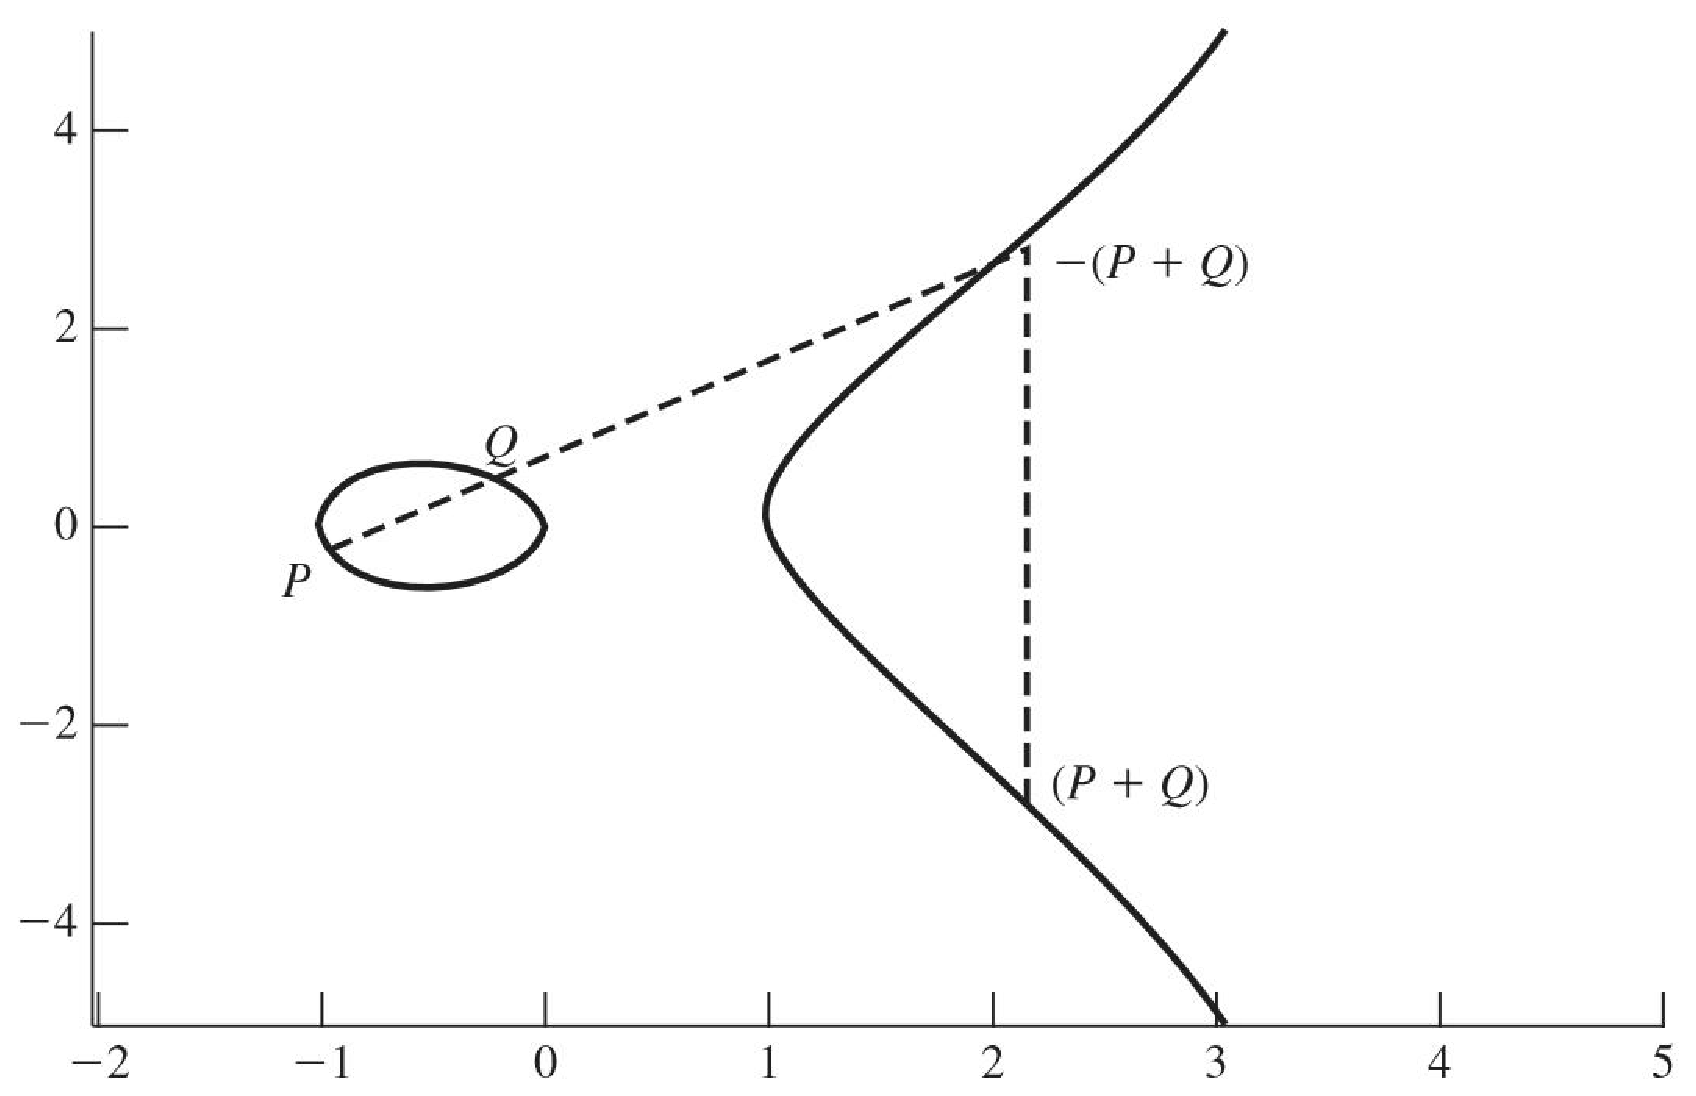
\includegraphics[width=7cm]{7-1.eps}
  \caption{$y^2=x^3-x$}
  \label{7-1}
\end{figure}

\begin{figure}[htbp]
  \centering
  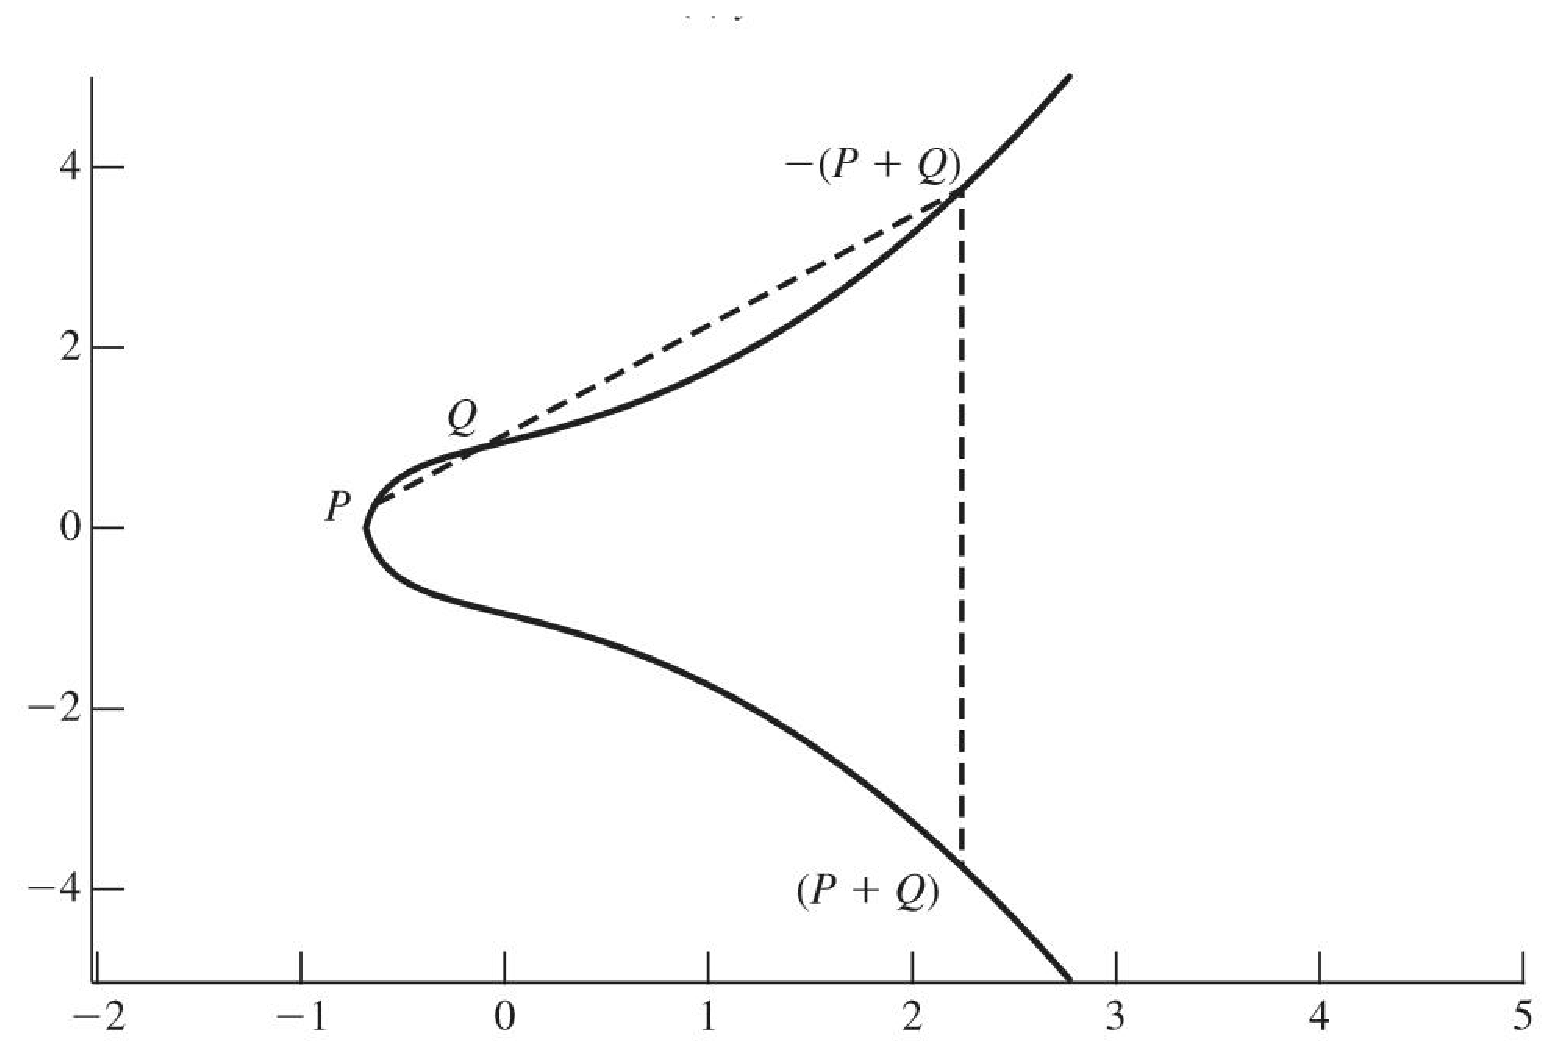
\includegraphics[width=7cm]{7-2.eps}
  \caption{$y^2=x^3+x+1$}
  \label{7-2}
\end{figure}

\textbf{Answer:}

We use the equations below.

\begin{equation}
y^2 = x^3 + ax + b
\end{equation}

\begin{equation}
4a^3 + 27b^2 \neq 0
\end{equation}

Then,
\begin{enumerate}
\item For $y^2 = x^3 - x$, we have $4(-1)^3 + 27(0) = -4 \neq 0$.
\item For $y^2 = x^3 + x + 1$, we have $4(1)^3 + 27(1) = 21 \neq 0$.
\end{enumerate}

\textbf{19.} What are the requirements for the use of a public-key certificate scheme?\\


\textbf{Answer:}

\begin{enumerate}
\item Any participant can read a certificate to determine the name and public key of the certificate's owner.
\item Any participant can verify that the certificate originated from the certificate authority and is not counterfeit.
\item Only the certificate authority can create and update certificates.
\item Any participant can verify the currency of the certificate.
\end{enumerate}

\textbf{20.} What are the essential ingredients of a public-key directory?\\

\textbf{Answer:}

\begin{enumerate}
\item The authority maintains a directory with a {name, public key} entry for each participant.
\item Each participant registers a public key with the directory authority. Registration would have to be in person or by some form of secure authenticated communication.
\item A participant may replace the existing key with a new one at any time, either because of the desire to replace a public key that has already been used for a large amount of data, or because the corresponding private key has been compromised in some way.
\item Periodically, the authority publishes the entire directory or updates to the directory. For example, a hard-copy version much like a telephone book could be published, or updates could be listed in a widely circulated newspaper.
\item Participants could also access the directory electronically. For this purpose, secure, authenticated communication from the authority to the participant is mandatory.
\end{enumerate}


\end{document}
